%UNIT 3: AN ANALYTIC APPROACH
%%%%%%%%%%%%%%%%%%%%%%%%%%%
%%%% Put the following at the top of each .tex file  %
\pagestyle{fancy}
\renewcommand{\theUnit}{3}
\ifthenelse{\isundefined{\UnitPageNumbers}}{}{\setcounter{page}{1}}
\rhead{Unit \theUnit: An Analytic Approach}
\lhead{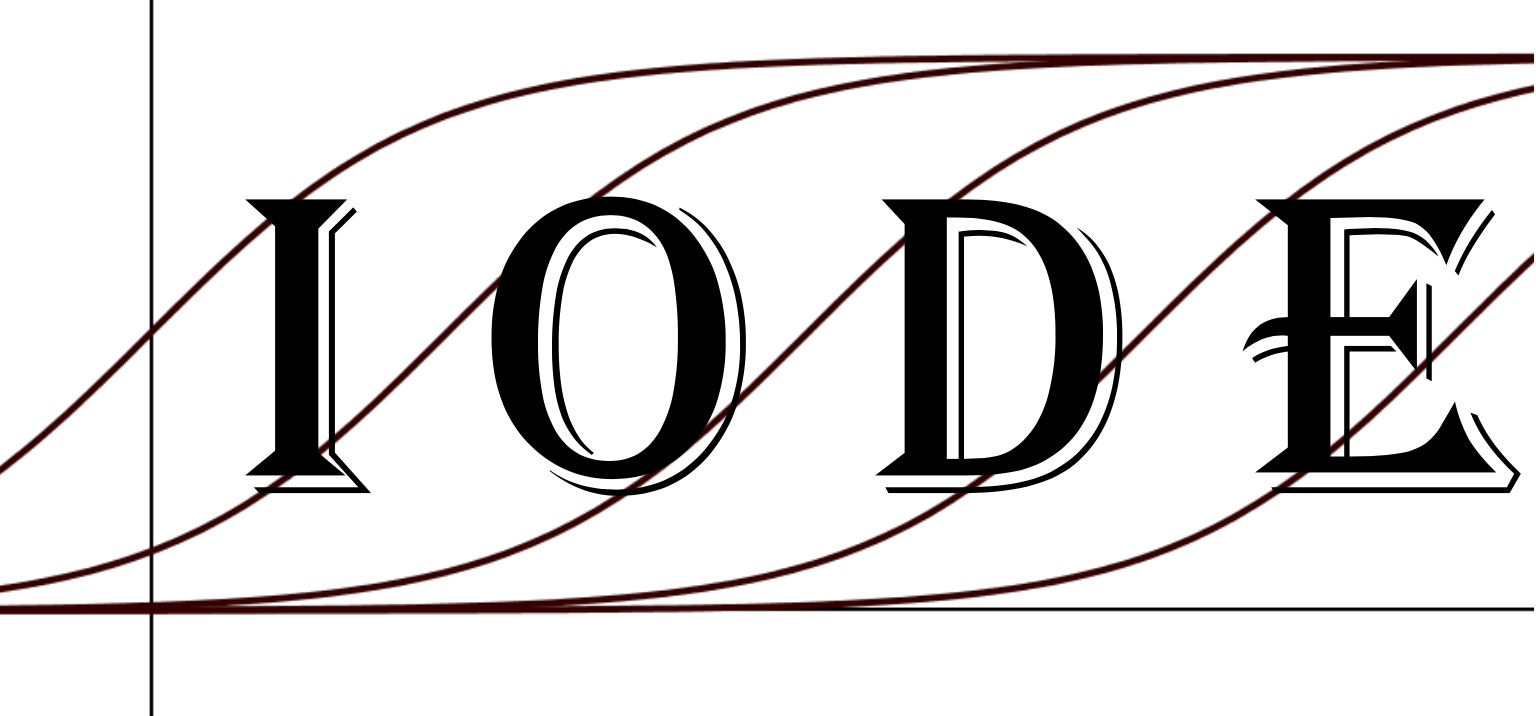
\includegraphics[width=1.25cm]{IODE-logo.png}}
\rfoot{\mypage}
\lfoot{}
\cfoot{}
\fancypagestyle{firstfooter}{\footskip = 50pt}
\renewcommand{\footrulewidth}{.4pt}
%%%%%%%%%%%%%%%%%%%%%%%%%%%
\vspace*{-20pt} \thispagestyle{firstfooter}
\pagebegin{Comparing Predictions}

Jerry and Tom are using the differential equation $\displaystyle\frac{dP}{dt} = 0.2P$ to make predictions about the number of a particular species of fish in Lake Michigan. They know that the initial population $P$ is 2 at time $t = 0$ (as before, think of 2 as scaled for say, 2,000 or 20,000).
 \vs
Although Jerry and Tom have the same goal (to obtain predictions for future fish population), they have different approaches to achieve this goal. 

\begin{itemize}
\item	Tom's approach is to create a graph of the number of fish versus time by connecting slope vectors tip-to-tail, where the rate of change is constant over some time interval, for example $\Delta t=0.5$. 
\item Jerry's approach is to create a graph of the number of fish versus time by using a continuously changing rate of change. 

\end{itemize}
\begin{enumerate}

\item Sketch Tom and Jerry's approaches below. Will these two approaches result in the same predictions for the number of fish in, say, $2.5$ years? If yes, why? If not, how and why will the graphs of their approaches be different?\label{03problem1}
\begin{center}
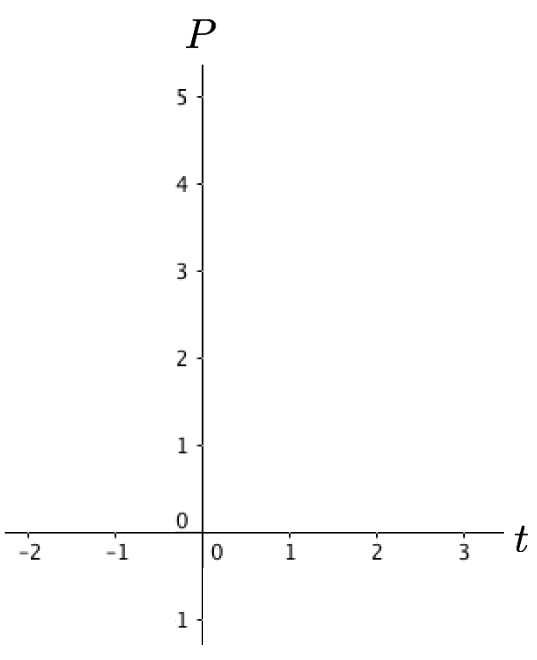
\includegraphics[width=3in]{03/03TomJerry.png}
\end{center}
\end{enumerate}
\clearpage

%%%%%%%%%%%%%%%%%%%%%%
\pagebegin{Separation of Variables}

\begin{enumerate}[resume]
\item	\textbf{Finding the exact solution}. Jerry's approach involves using a continuously changing rate of change, which corresponds to finding an ``exact solution.'' \label{03problem2}
\begin{enumerate}

\item	Why do you think the phrase ``exact solution'' is used to describe the result of Jerry's approach? Explain why it is appropriate to describe the result of Tom's approach as an ``approximate solution''. \label{03problem2parta}

\vfill
\item Use the chain rule to write down, symbolically, the derivative with respect to $t$ of $\ln (P)$, where $P$ is shorthand for $P(t)$. \label{03problem2partb}
\end{enumerate}
\vfill

\clearpage

Next you will learn a technique for finding the exact solution corresponding to Jerry's approach. We begin by considering the chain rule.

\begin{enumerate}[resume]
\item	 The following is a method to find the analytic solution to $\displaystyle\frac{dP}{dt}= 0.2P$. For now assume that $P > 0$. This assumption corresponds to the population growth context and it will make the algebra easier and hence the underlying idea clearer.  \label{03problem2partc}
 
\end{enumerate}

\begin{center} \renewcommand{\arraystretch}{1.5}
\newcolumntype{V}{>{\centering\arraybackslash} m{.5\linewidth} }
\begin{tabular}{|p{2in}|V|}
\hline

Divide both sides of \newline $\frac{dP}{dt}=0.2P$ by $P$ &
{} \\
{} & {} \\
\hline

Replace $\frac{1}{P}\frac{dP}{dt}$ with $\left[ \ln(P)\right]'$ & 
{} \\
{} & {} \\
\hline
	 
Write integrals with respect to $t$ on both sides & 
\\{} & {} \\ 
\hline
	 
Apply the Fundamental Theorem of Calculus to integrate both sides & 
\\{} & {} \\
\hline	 

Solve for $P$ (and remember that $P$ is actually a function, $P(t)$) & 
\\{} & {} \\
\hline

Show that $P$ can be written as $P(t) = ke^{0.2t}$ & 
\\{} & {} \\
{} & {} \\
\hline
\end{tabular} \end{center}

The end result, $\displaystyle P(t)=ke^{0.2t}$ is called the \textbf{general solution} because it represents all possible functions that satisfy the differential equation. We can use the general solution to find any \textbf{particular solution}, which is a solution that corresponds to a given initial condition.

\item	Use the same technique to find the general solution to $\displaystyle\frac{dy}{dt}=\frac{t}{3y^2}$. The first step is done for you. \label{03problem3}
\vs
$\displaystyle 3y^2\frac{dy}{dt}=t$
\vfill

\clearpage

\item In practice, we often circumvent explicit use of the chain rule and instead use a shortcut to more efficiently find the general solution. The shortcut involves treating the derivative $\frac{dP}{dt}$ as a ratio and ``separating'' the $dP$ and $dt$. In the table below, follow the instructions to see how the shortcut works, using again the equation $\displaystyle\frac{dP}{dt} = 0.2P$. (See \href{http://kevinboone.me/separation_variables.html}{\underline{http://kevinboone.me/separation\textunderscore variables.html}}) for a nice explanation of the shortcut). \label{03problem4}
\vs

\begin{center}\renewcommand{\arraystretch}{1.5}
\newcolumntype{V}{>{\centering\arraybackslash} m{.5\linewidth} }
\begin{tabular}{|p{2.5in}|V|}
\hline
`Separate' the $dP$ from the $dt$ so that $dP$ and $P$ are on the same side. (If there are $t$'s in the equation they must go on the same side as $dt$.)
	  &
{} \\\hline

Integrate both sides of the equation (one side with respect to $P$, the other with respect to $t$)	  &
{} \\\hline

Continue as before to arrive at a solution of the form $P(t)=\underline{\hskip1cm}$	 	  &
{} \\
{} & {} \\
{} & {} \\
{} & {} \\
{} & {} \\
{} & {} \\
{} & {} \\
{} & {} \\ \hline
\end{tabular}
\end{center}

\item	Use the shortcut to find the general solution to  $\displaystyle \frac{dy}{dt}=\frac{t}{3y^2}$. \label{03problem5}
\vfill

\clearpage

\item	A differential equation together with an initial condition is called an \textbf{Initial Value Problem} (IVP). To solve an IVP one first must find the general solution and then use the initial condition to find the particular solution corresponding to the initial condition. \label{03problem6} \\ Solve the following IVP:    
\[ \frac{dy}{dt}=\frac{t}{y}\hspace{0.5in} y(2)=-1\]
\vfill

\begin{enumerate}
\item	 For what values of $t$ is your solution valid? Why? \label{03problem6parta} 
\vskip1cm

\item Check to see that your {particular} solution ``fits'' the differential equation by substituting the solution and its derivative into the original differential equation. \label{03problem6partb} 
\vfill

\item	Use the GeoGebra applet, \href{https://ggbm.at/SbHk2n4H}{\underline{https://ggbm.at/SbHk2n4H}}, to check to see that your specific solution ``fits'' the differential equation by plotting the slope field and then plotting the graph of the solution on top of the slope field. Explain how this relates to Jerry's approach. \label{03problem6partc}

\vspace{-.25in}\hspace{-.75in}
\includegraphics[width=0.5in]{03/03IVPQR.png}
\vfill

\item Consider a different initial condition, $y(2) = 0$, to the same differential equation, $\displaystyle\frac{dy}{dt}=\frac{t}{y}$. Note that even though $\displaystyle\frac{dy}{dt}$ is undefined when $y = 0$, our separation of variables technique can still yield something meaningful. What should the solution to this IVP be? \label{03problem6partd} 
\vfill
\end{enumerate}

\end{enumerate}

\clearpage

%%%%%%%%%%%%%%%%%%
\pagebegin{Making Connections}

\begin{enumerate}[resume]
\item For the first slope field for $\frac{dL}{dt} = 0.5(1 - L)$ on the following page,\label{03problem7}
\begin{enumerate}

\item	Using Jerry's approach, sketch as accurately as possible a graph of the solution with initial condition $L(0) = 1/3$. \label{03problem7parta}
\item	Make a copy of this sketch on a transparency. \label{03problem7partb}
\item	If you wanted to obtain the graph of the solution with initial condition $L(0) = 1/2$, how, if at all, might you move the copy of your graph with initial value 1/3 so that it is now a graph of the solution with initial value 1/2? What feature of the differential equation justifies your approach? \label{03problem7partc}
\item	Find the general solution for $\displaystyle\frac{dL}{dt}= 0.5(1-L)$ and explain how your results from part \ref{03problem7partc} can be understood from the general solution.\label{03problem7partd}
\vfill	

\end{enumerate}
\item	For the second slope field for $\frac{dh}{dt} = -t + 1$ on the following page,\label{03problem8}
\begin{enumerate}
\item	Using Jerry's approach, sketch as accurately as possible a graph of the solution with initial condition $h(0) = 1/2$. \label{03problem8parta}
\item	Make a copy of this sketch on a transparency. \label{03problem8partb}
\item	If you wanted to obtain the graph of the solution with initial condition $h(0) = 1$, how, if at all, might you move the copy of your graph with initial value $1/2$ so that it is now a graph of the solution with initial value 1? Explain your idea and provide reasons for why your idea makes sense. \label{03problem8partc}
\item	Find the general solution for $\frac{dh}{dt} = -t + 1$ and explain how your results from part \ref{03problem8partc} can be understood from the general solution. \label{03problem8partd} \vfill
\end{enumerate}

\item  Give an example of a differential equation where neither of your ideas from \ref{03problem7partc} and \ref{03problem8partc} will work and provide reasons for your response.\label{03problem9}\vfill
\end{enumerate}

\clearpage

\begin{center}
\textbf{Slope Field} for $\displaystyle\frac{dL}{dt} = 0.5(1 - L)$

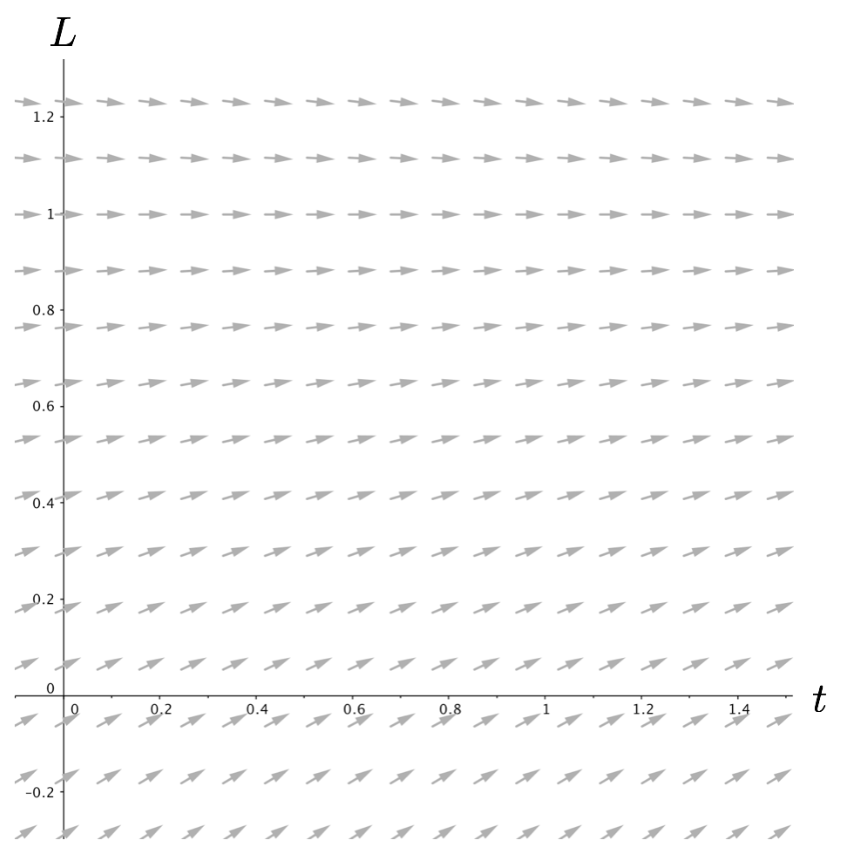
\includegraphics[width=4in]{03/03SlopeField1.png}

\vspace{.5cm}
\textbf{Slope Field} for $\displaystyle\frac{dh}{dt} = -t + 1$

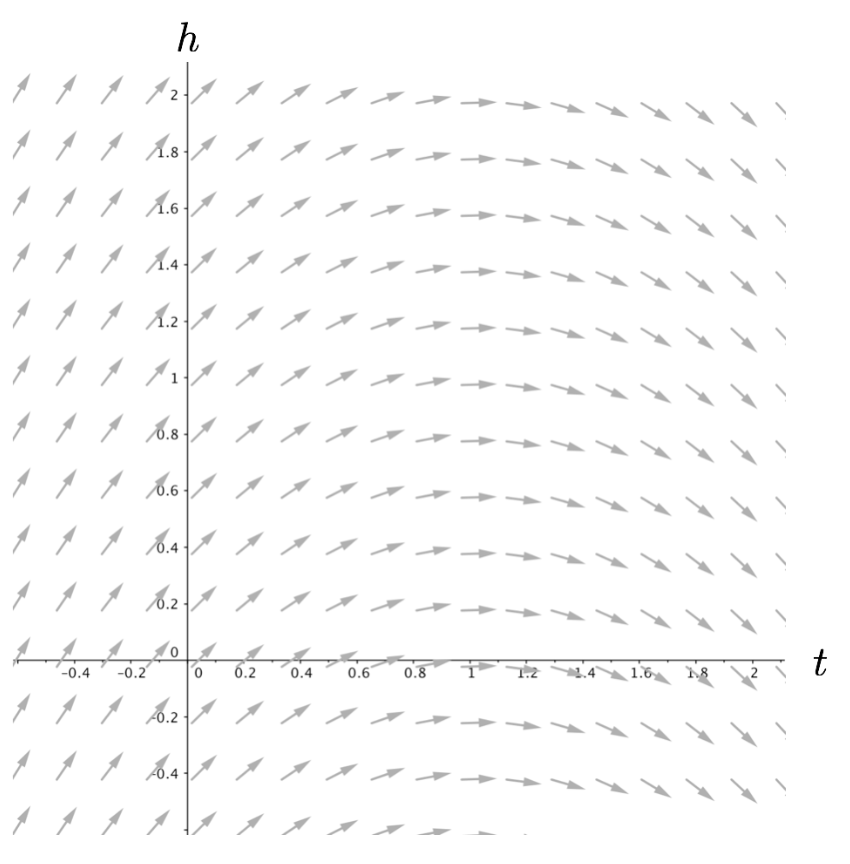
\includegraphics[width=4in]{03/03SlopeField2.png}\\
\end{center}

\clearpage

%%%%%%%%%%%%%%%%%%%%%%%%%%%%%%%%%%%%%%
\pagebegin{Homework Set 3}
\begin{enumerate}

\item When you solve an equation such as $x^2-3=1$ , you get two numbers $x=2$ and $x= -2$.  When you solve a differential equation, what do you get? \label{03HWproblem1}

\item Find the general solution to the following differential equations. \label{03HWproblem2}

\begin{enumerate}
\item $\displaystyle \frac{dy}{dt}=t^4y$
\item $\displaystyle \frac{dy}{dt}=2y+1$
\item $\displaystyle \frac{dy}{dt}=t\sqrt[3]{y}$
\item $\displaystyle \frac{dy}{dt}=\frac{t}{y+1}$
 \item $\displaystyle 2\frac{dy}{dx}=xy(x+1)$
\end{enumerate}
	 
\item	Find the particular solution to the following initial value problems. \label{03HWproblem3}
\begin{enumerate}
\item $\displaystyle \frac{dy}{dt}=\frac{-t}{y}, \qquad y(0)=4$
\item $\displaystyle \frac{dy}{dt}=-\sqrt[3]{y}, \qquad y(0)=27$
\item $\displaystyle \frac{dy}{dx}=\frac{x(y-2)}{x^2+4}, \qquad y(1)=5$
\end{enumerate}
	 
\item	Develop a differential equation where $y(t) = 6$ is a solution function but $y(t) = 8$ is not a solution function. Explain why your differential equation meets both of these criteria. \label{03HWproblem4}

\item Denise has created the following graph to go along with the rate of change equation $\frac{dP}{dt}=0.2P$. \label{03HWproblem5}
\begin{center}
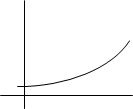
\includegraphics[]{03/03Denise.png}
\end{center}
What is this a graph of? Label the axes and explain your reasoning.

\clearpage

\item Cornelia is working with the differential equation $\displaystyle\frac{dy}{dt}= y - t$.  She has no method like separation of variables to use but still needs to a way to figure out which, if any, of the following functions are solutions to $\displaystyle\frac{dy}{dt}= y - t$. \label{03HWproblem6}
\[
\text{(i) }y(t)= t + 2 \hspace{.75in} \text{(ii) }y(t)= e^t-1 \hspace{.75in} \text{(iii) }y(t) = e^t  + t + 1 \hspace{.75in} \text{(iv) }y(t) = t
\]
  
\begin{enumerate}
\item Read the differential equation $\displaystyle\frac{dy}{dt}= y - t$ with {\em meaning}. Write down exactly how you would read the equation with meaning. Recall {\em reading with meaning} was discussed in Unit 1.
\item	Explain how Cornelia can use a slope field to determine which, if any, of these functions are solutions to the differential equation, $\displaystyle\frac{dy}{dt}= y - t$. 
\item	Use what it means to be a solution to a differential equation to determine which, if any, of these functions are solutions to $\displaystyle\frac{dy}{dt}= y - t$.  Show all work.
\end{enumerate}

\item
\begin{enumerate}
\item Go to the glossary and identify all terms that are relevant to this unit and list those terms here.
\item Are there other vocabulary terms that you think are relevant for this unit that were not included? If yes, list them.
\end{enumerate}

\end{enumerate}

